\documentclass[12pt, letterpaper]{article}

\usepackage{amsmath} % needed for including equations
\usepackage[margin=1in]{geometry} % sets the margins to 1in
\usepackage{graphicx} % needed for figures
\graphicspath{{./figures/}} % allows figures to be placed in a different folder
\usepackage[hang,small,bf]{caption} % sets the style on the figure captions
\usepackage{epstopdf} % converts eps files to pdf to display in the latex document



\begin{document}

\begin{titlepage}

\begin{center}

\vspace*{\fill}

\vspace{0.5in}

% Insert your title here
{ \LARGE \bfseries Precision Maritime Landing of Quadrotor UAS On Small Sea Vessels}\\[.25in]

\large
by\\[.25 in]
% Change your name here
Jesse S. Wynn\\[1in]

A prospectus submitted to the faculty of\\
Department of Mechanical Engineering\\
Brigham Young University

\vspace{1in}

\today

\vspace*{\fill}

\end{center}

\end{titlepage}

\thispagestyle{empty}

\begin{center}
\vspace*{\fill}

\begin{figure}[htbp] %  figure placement: here, top, bottom, or page
   \centering
   
\includegraphics[width=2.5in]{byume_logo_clear.jpg} 
\end{figure}

\vspace{0.5in}

\Large{Prospectus Approval}\\[0.5in]

\end{center}

\hspace*{.47in}
\begin{minipage}[c]{5.25in}

\normalsize

Prospectus submitted by:

\vspace{.5in}

\makebox[2in]{\hrulefill} \hspace{1in} \makebox[2in]{\hrulefill}

% Change your name here
\parbox[b]{3in}{Your name} \, Date
\vspace{0.5in}

This prospectus has been approved by each member of the Graduate Committee:
\vspace{0.5in}

\makebox[2in]{\hrulefill} \hspace{1in} \makebox[2in]{\hrulefill}

\parbox[b]{3in}{Committee Member - Chair} \, Date
\vspace{0.4in}

\makebox[2in]{\hrulefill} \hspace{1in} \makebox[2in]{\hrulefill}

\parbox[b]{3in}{Committee Member} \, Date
\vspace{0.4in}

\makebox[2in]{\hrulefill} \hspace{1in} \makebox[2in]{\hrulefill}

\parbox[b]{3in}{Committee Member} \, Date

\end{minipage}

\vspace*{\fill}

\pagebreak

\setcounter{page}{1}

\section{Problem Statement}

Thanks to the rapid advancement of quadrotor unmanned aircraft systems (UAS) technology, applications in maritime environments and conditions are becoming more viable.  A critical capability for nearly all UAS at sea is the ability to autonomously and accurately land on moving platforms, such as a ship deck \cite{Herisse2012}.  A variety of algorithms for shipboard landing have already been developed--many of which incorporate a downward-facing vision sensor to track some kind of marker on deck \cite{Truskin2013} \cite{Kong2014}.  A widespread weakness of current landing techniques however, is that they usually require good visibility, and relatively calm sea state to operate reliably \cite{Tan2016}. Also, the assumption is often made that the ship is a large vessel and is therefore much less agile than the UAS, and less affected by turbulent seas \cite{Ling2014}.  Given that favorable visibility and sea state may, at any time not be found on actual seas, and that the resulting challenges are further compounded when the sea vessel is small, the problem of enhancing quadrotor UAS maritime landing capabilities for small vessels is motivated.  

%The objective of this proposed research is not to create a new landing algorithm from scratch, but rather to understand how the integration and fusion of additional sensor measurements can enable current methods to operate reliably in a greater range of conditions and sea states.

The objective of this proposed research is not to create a new landing algorithm entirely from scratch, but rather to explore how the addition and fusion of additional sensors and measurements can enable current techniques to operate reliably for small vessels in a broader range of conditions.  Of particular interest is the ability to operate in low-light environments, and in conditions where ship deck motion (heave, roll, pitch) is relatively large.


\section{Background}

%Detonation is a pressure-gain, near constant-volume combustion %process. The pulse detonation cycle consists of three main %events: fill, fire, and purge. Figure~\ref{fig:PDEcycle} %visually shows the pulse detonation cycle described below.

Current vision-based approaches to quadrotor UAS shipboard landing typically segment the maneuver into separate stages, guided by a state machine.  An outline that briefly describes each of these stages generally, is given below.   

\begin{enumerate}
\item Global Interception.  In this stage, the UAS navigates to within a near vicinity of the ship using its own global positioning capabilities, and known GPS data from the ship.  The goal of this stage is to bring the UAS and ship into close enough proximity for the UAS to be able to spot the landing marker on deck using on-board vision sensors.
\item Relative Interception.  In this stage, the UAS position controller switches from GPS commands to relative commands based on the position and orientation of the landing marker in the image frame.  In this stage the UAS may also begin tracking the heave motion of the ship, attempting to maintain constant height above the ship deck.
\item Initial Descent.  The goal of this stage is to slowly reduce the height distance between the UAS and the ship deck while keeping the UAS laterally positioned above the marker.
\item Touchdown. In this stage, the UAS is close to the ship deck and the edges of the marker are leaving the FOV of the vision sensor(s).  The goal of this stage is to achieve a gentle touchdown on the ship deck by relying on any relative sensor data that is still available, and/or on-board predictions about the ship deck motion.
\end{enumerate}

%\begin{figure}[htbp] %  figure placement: here, top, bottom, or page
%   \centering
%   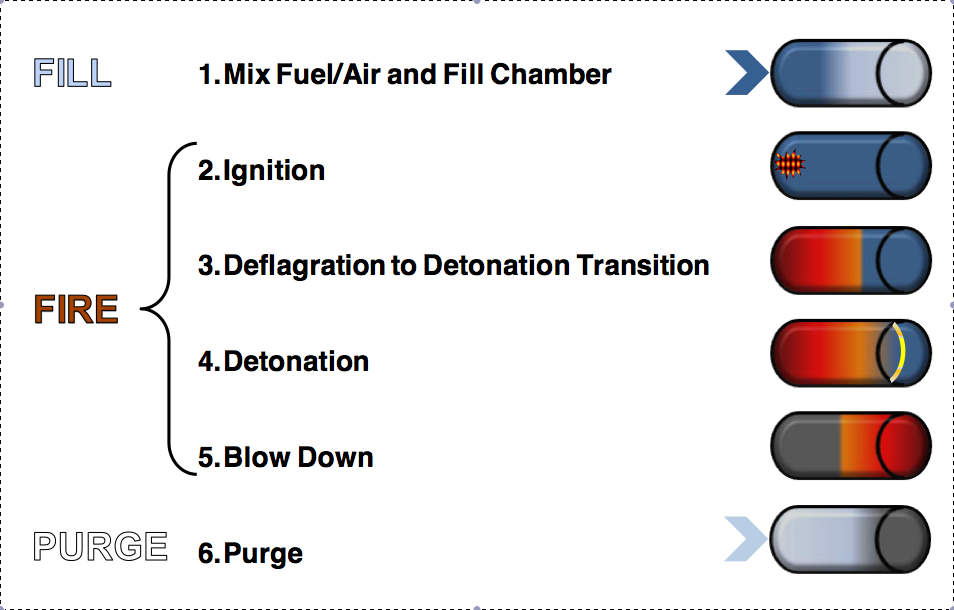
\includegraphics[trim = 5mm 5mm 5mm 5mm,clip,width=4in]{PDEcycle.png} 
%   \caption{The PDE cycle as presented by Rouser et. al.}
%   \label{fig:PDEcycle}
%\end{figure}

%Garratt, Pota, Lambert et al. 2009
In 2009, Garratt et. al. \cite{Garratt2009} detailed a shipboard landing method for autonomous collective pitch helicopters that used a digital camera and a laser range finder pointed at a spinning mirror to supply data for estimating the relative position and motion of the ship deck.  Flight test results showed that their system was able to estimate the relative roll and pitch angles, as well as height distance between the helicopter and the simulated ship deck to a high degree of accuracy.  Their results however only demonstrated the capabilities of their measurement and estimation system and did not demonstrate the actual ability to execute a successful landing maneuver.
  
%Ling, Chow, et al. 2014
In 2014 Ling et. al. \cite{Ling2014} presented a low-cost method for performing autonomous maritime landings with small VTOL aerial vehicles.  Their sensing system consisted of a uEye camera on-board the VTOL and an AprilTag fiducial target on the simulated ship deck.  Their method demonstrates the ability to accurately track the position of the shipboard landing target, but more work would be needed before a robust estimate of the ship deck attitude could be estimated.  Further, their system was constructed around a highly simplified model for the ship dynamics and would likely breakdown if actual ship motion were to be more extreme.   

%probably need to add some more background references here

From this brief survey of the current research, it can be seen that although various and significant contributions have been made in the field of autonomous shipboard landing, there is still great opportunity for continued research.

\section{Research Objectives}

To successfully complete this proposed research, the following objectives will be accomplished:


\begin{itemize}

	\item Build up a simulation environment that models and controls a generic quadrotor UAS, and also includes a model of a ship deck whose motion can be driven based on a given sea state.

	\item Implement an existing vision-based landing approach in simulation to be used as a baseline for shipboard landing performance.  

	\item Augment the simulation by modeling additional sensor data from the UAS and/or ship that can be used to enable successful autonomous landings in a wider range of sea conditions.

	\item Based on the most effective approach found through simulation, implement the solution in hardware on an actual quadrotor with onboard sensors and ship-based sensors.
	
	\item Perform flight test demonstrations and gather test data to showcase the effectiveness of the solution that has been developed.

\end{itemize}

\section{Proposed Research}

To address the problem at hand, a multi-phase approach will be used.  Research work will commence by first identifying a suitable and somewhat generic controls framework that can be used to accomplish a vision-based shipboard landing.  This framework will then be implemented and tested in simulation using MathWorks\textsuperscript{\textregistered} MATLAB and SIMULINK.  To keep things simple to begin with, a proportional integral derivative (PID) controller will be implemented for the Quadrotor UAS.  The Extended Kalman Filter (EKF) will be used to generate state estimates for the UAS, and will be augmented to take in additional measurement inputs from the vision system in order to generate estimates for the ship deck attitude.  Once functional in simulation, tests will be performed to evaluate the performance and limitations of the vision-based landing approach. 

Brigham Young University, and specifically the MAGICC Lab, has a strong background in the field of 'Relative Navigation' for UAS \cite{Leishman2013}.  Though the shipboard landing problem is significantly different than the relative navigation work that has been previously performed here, successful shipboard landing requires a form of relative navigation, and can likely draw on some of the relative navigation work that has already been done.  In the current relative navigation problem, measurements between the static surroundings and the dynamic UAS are taken to estimate the relative position and velocities of the UAS.  If we now flip the problem by assuming that the UAS is pseudo-stationary (i.e. its movement is small and its position is known thanks to GPS), we would like to explore the possibility of taking similar measurements to estimate the state of the dynamic surrounding (i.e. the ship deck). In the current relative navigation problem, an accurate estimate of the UAS' state is aided significantly by measurements from an on-board IMU. Similarly, we would like to research the contribution that a ship-based IMU can offer to enable a more robust shipboard landing solution.

Though much of this proposed research will begin in simulation, the resultant methods and solutions that are discovered are planned to be implemented in hardware flight tests.  Testing in hardware will require a quadrotor UAS to be procured and assembled, and will also require a ship deck motion emulator to be fabricated.  The UAS will be comprised of standard hobbyist equipment for the airframe and propulsion system, and the ship deck emulator will similarly be fabricated using off-the-shelf components.  Autopilot capabilities for the UAS will be enabled through the use of a ROSflight flight controller paired with an on-board computer that will run the autopilot control loops in Robot Operating System (ROS).  The ship deck emulator is planned to have its own GPS receiver and IMU unit.  Communication of sensor measurements and/or state estimates from the ship deck emulator to the UAS are planned to be communicated over a local WiFi network.  At all times during flight test operations the UAS will be controllable through a ground-station computer, and a safety pilot will be present to take manual control of the UAS at any moment.  

\begin{figure}[htbp] %  figure placement: here, top,  bottom, or page
   \centering
   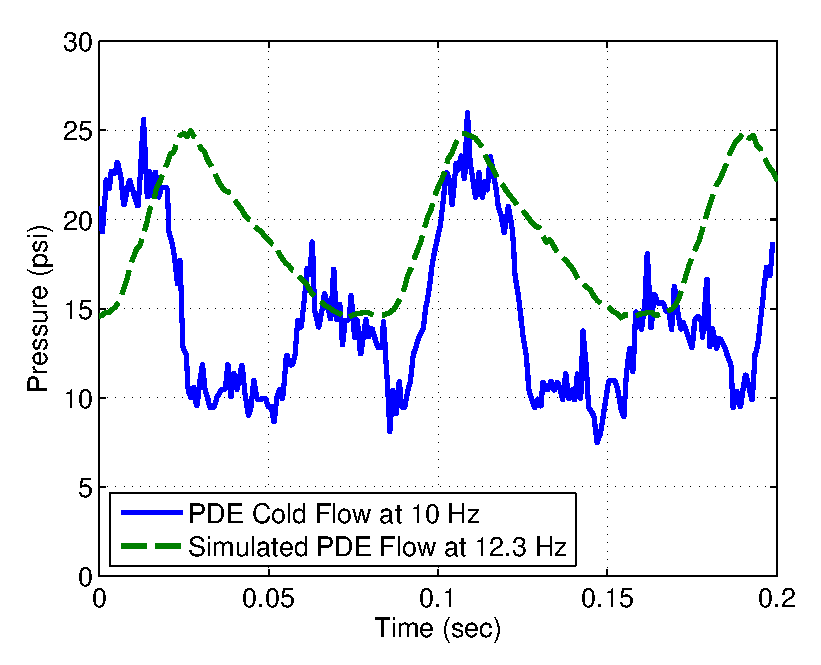
\includegraphics[trim = 0mm 0mm 0mm 0mm,clip,width=4in]{pressure.eps}
   \caption{Comparison of actual and simulated PDE flow. The solid blue line is the turbine inlet pressure for cold flow as presented by Rouser et. al.. The dashed green line is the exit pressure from a valve rotated at 12.3~Hz. The peaks are not aligned due to the different operating frequencies. This figure shows that a rotating ball valve can be used to qualitatively approximate PDE flow through a turbine.}
   \label{fig:pressurecomparison}
\end{figure}

The experimental apparatus will have instrumentation to measure pressures, temperatures, and mass flow.
%The pressures and temperatures will be measured at the turbine and compressor inlets and outlets. Pressures will be measured using pressure transducers and temperatures using thermocouples. The thrust will be measured using an air bearing system to decrease friction and a strain gauge. The mass flow into the compressor and turbine will be measured.
Turbine power will be measured using the compressor work. Exact power measurement is not necessary since a comparison will be made on the same equipment and not with independently collected data.

Experimental data will be used to compare steady and pulsed flow. Comparisons will be made using specific power, turbine efficiency, and a turbine map. Specific thrust and power will both be calculated by dividing the respective quantities by the mass flow rate through the turbine. The conventional methods used to calculate turbine efficiency are not adequate due to the unsteady flow conditions. A method to include the unsteady effects in the calculation of efficiency is still being investigated.

An example of an equation is shown in Equation~\ref{eq:efficiency}.

\begin{equation}
\eta_t = \cfrac{\dot W_c + \dot W_{fric}}{\dot m c_p \left[ 1 - \left( \cfrac{p_{t5}}{p_{t4}} \right)^\frac{\gamma - 1}{\gamma} \right]}
\label{eq:efficiency}
\end{equation}

%Flack \cite{flack:2008fundamentals-of} presents a method to create a turbine map. Both turbine pressure ratio and efficiency can be expressed as functions of corrected mass flow and rotational speed as shown in Equations~\ref{pressure_ratio} and~\ref{efficiency_function}.
%
%\begin{equation}
%\frac{p_{t4}}{p_{t5}} = \mathscr{F} \left\{ \frac{\dot m \sqrt{\theta_{t4}}}{\delta_{t4}}, \frac{N}{\sqrt{\theta_{t4}}} \right\} = \mathscr{F} \left\{ \dot m_{c4}, N_{c4} \right\}
%\label{pressure_ratio}
%\end{equation}
%%
%\begin{equation}
%\eta = \mathscr{G} \left\{ \frac{\dot m \sqrt{\theta_{t4}}}{\delta_{t4}} , \frac{N}{\sqrt{\theta_{t4}}} \right\} = \mathscr{G} \left\{ \dot m_{c4}, N_{c4} \right\}
%\label{efficiency_function}
%\end{equation}
%%
%where
%\[\delta_{t4} = p_{t4}/p_{stp}\]
%and
%\[\theta_{t4} = T_{t4}/T_{stp}\]
%%
%Lines of constant corrected speed and efficiency will then be plotted on an axis of pressure ratio versus corrected mass flow.

\section{Anticipated Contributions}

As a result of this research, there will be an improved understanding of the effect of unsteady, pulsed flow through a turbine. A direct comparison will be made between steady and unsteady flow through an axial turbine without any bypass flow. This direct comparison has not been previously performed. Possible publications from this research include presenting at the ASME Turbo Expo, submitting to the ASME Journal of Turbomachinery, presenting at the AIAA Aerospace Science Meeting, or other conferences and journals. This research is sponsored by Innovative Scientific Solutions, Inc. through an Air Force contract.


\pagebreak

\bibliographystyle{IEEEtran}
\bibliography{library}

\end{document}